\section{Graphical user interface (GUI)}
\label{sec_GUI}

\begin{figure}
   \centering
   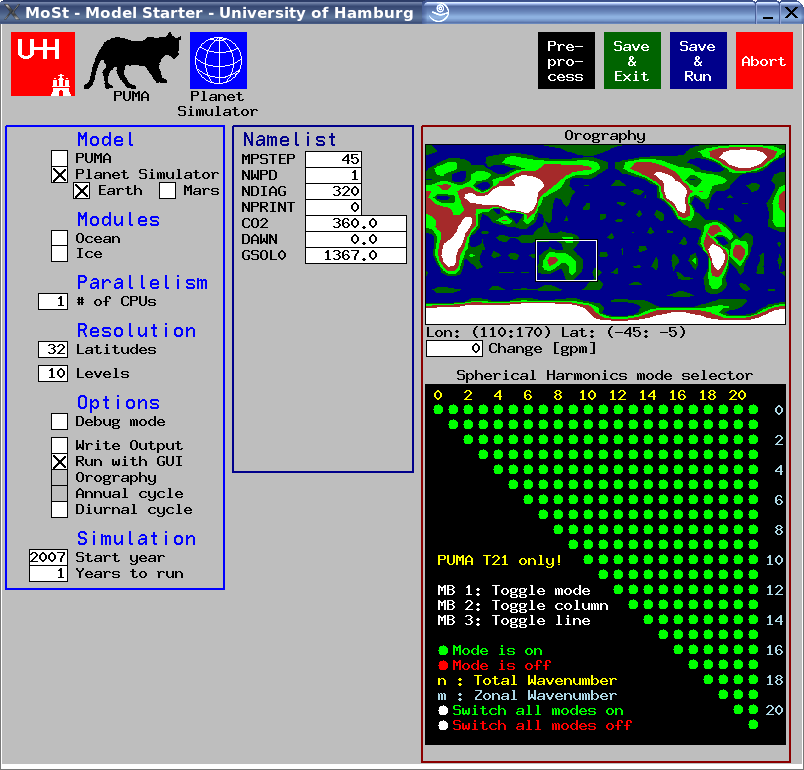
\includegraphics[width=8.5cm]{Pics/mostsnap}
   \caption[]{Screenshot of Model Starter (MoSt)}
   \label{mostsnap}
\end{figure}

The {\model} may be used in the traditional fashion,
with shell scripts, batch jobs, and network queuing 
systems. This is acceptable for long running simulations
on complex machines and number-crunchers, like vector-
computers, massive-parallel-computers and workstation clusters.
There is now, however, a much more convenient method by using
a graphical user interface (GUI) for model setup with parameter configurations
and for interaction between user and model.


The {\model} is configured and setup by the first
GUI module named MoSt (Model Starter, screenshot in \ref{mostsnap}). 
MoSt is the fastest way to get the
model running. It gives access to the most important parameters of
the model preset to the most frequently used values.
The model can be started with a mouse click on the button
labelled "Save \& Run" either with the standard paramater setting
or after editing some of the parameters in the MoSt window.
Some parameters, like horizontal and vertical resolution,
or the number of processors, require the building
(compile, link and load) of new executables. MoSt achieves
this by generating and executing build scripts,
that perform the necessary code changes and
create the required executable.
Other parameters define startup- and
boundary conditions or settings for parameterisations.
They can be edited in MoSt and, after a check for
correct range and consistency with other parameters,
are written to the model's namelist file.

Depending on all settings
MoSt generates a runscript for the simulation.
The user has the choice of leaving MoSt and
continue with the simulation under control of a GUI
right away, or to exit MoSt with the scripts prepared
to run. The second alternative is useful for users, who
want to modify the setup beyond the scope of MoSt
or want to run the Planet Simulator without GUI.

There's also a simple graphical editor for topograpy.
Check the box Orography and then use the mouse to mark
rectangular areas in the topography display.
Enter a value for rising (positive) or lowering the area
and press the button labelled {\bf Preprocess}.
The preprocessor will be built and executed, a new
topography will be computed and written to a start file.

Another editor is the mode editor for spherical harmonics.
Green modes are enabled, red modes are disabled.
This feature can be used to make runs with only certain
modes of spherical harmonics being active.
MB1, MB2, MB3 refer to the left, middle, and right mouse
button. You may toggle individual modes or whole lines
and columns. Currently this mode editor can only be used
for {\model} in the T21 resolution.

\begin{figure}
   \centering
   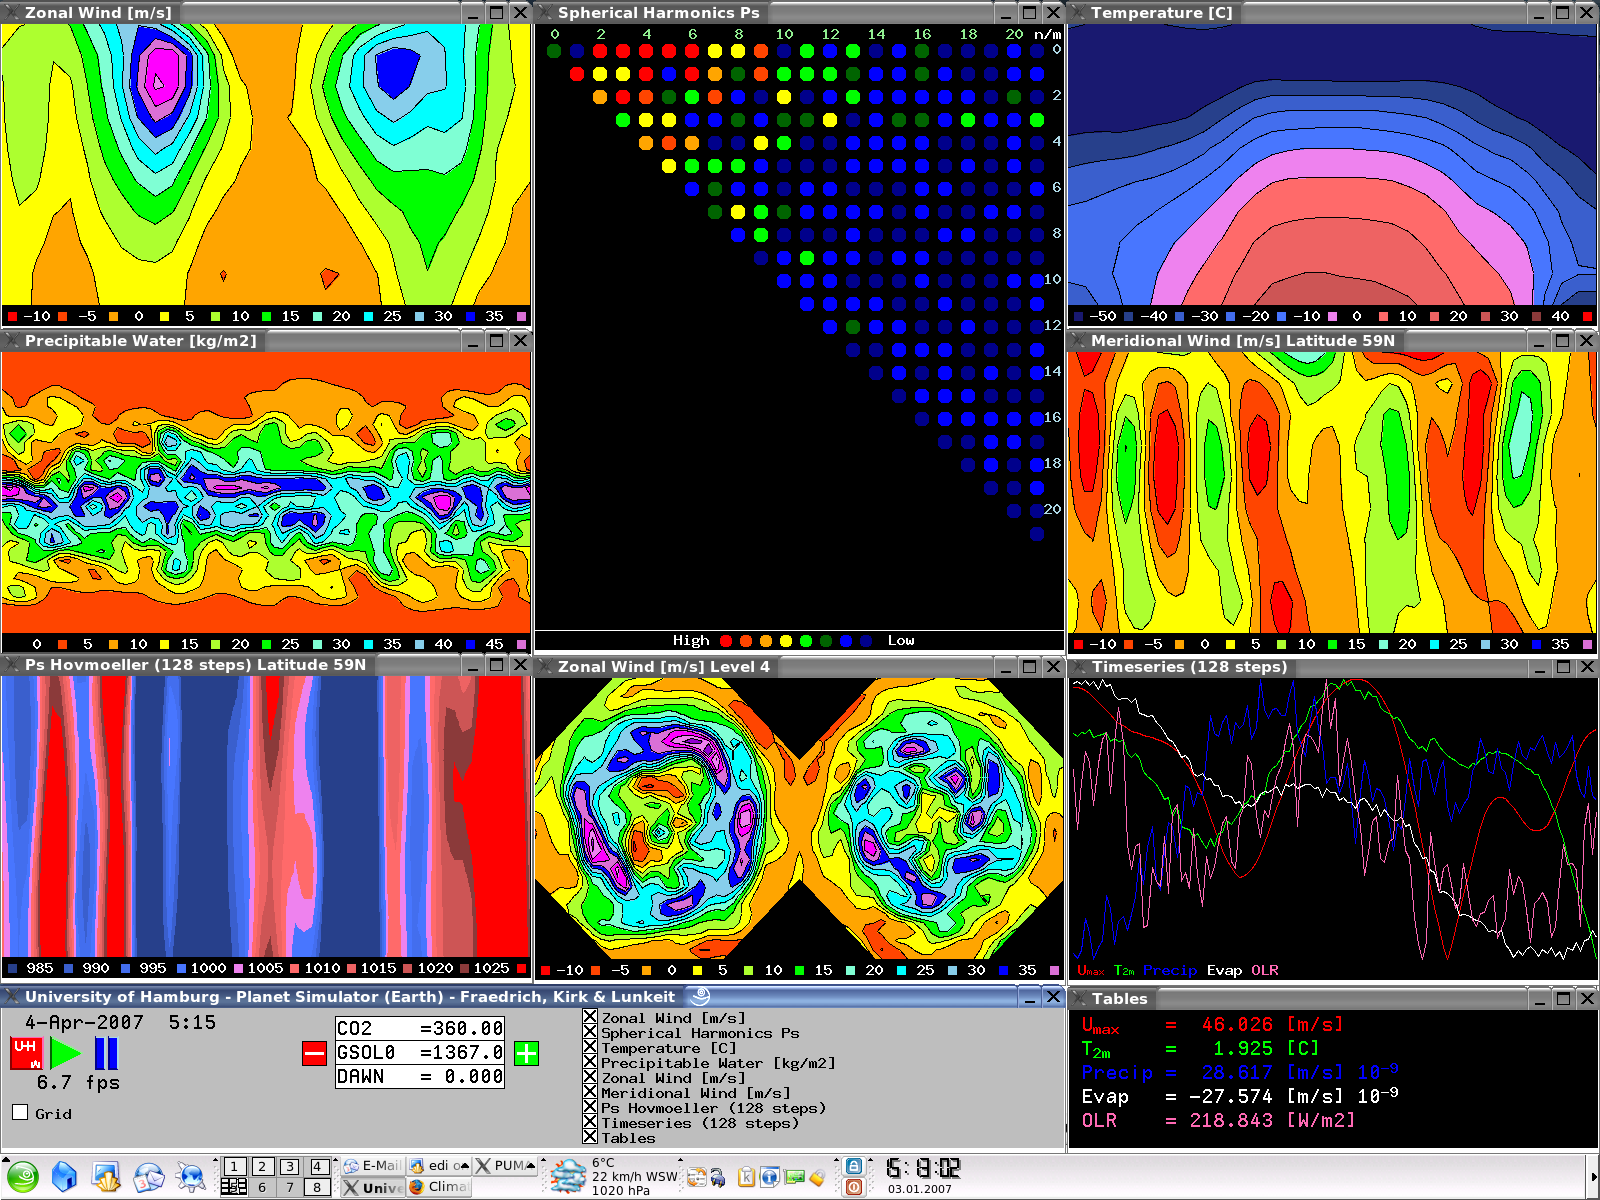
\includegraphics[width=8.5cm]{Pics/guisnap}
   \caption[]{Screenshot of Graphical User Interface (GUI)}
   \label{guisnap}
\end{figure}

The GUI for running the {\model}
(screenshot in \ref{guisnap})
has two main purposes. The first one is to display
model arrays in suitable representations.
Current implementations are:
\begin{itemize}
\item{Zonal mean cross sections}
\item{Horizontal global fields in cylinder projection}
\item{Horizontal global fields in polar projection}
\item{Time-longitude (Hovmoeller) diagrams}
\item{Amplitudes of coefficients of spherical harmonics}
\item{Time series}
\item{Numerical values}
\end{itemize}

In case of horizontal global grids pressing the MMB (Middle Mouse Button)
toggles between cylinder and polar projection. If the grid is
just one level from many of a three dimensional field like u or v,
the level shown can be decreased by the LMB or increased by the RMB.
For Hovmoeller and longitude height sections the LMB and RMB can
be used to select the latitude.

The second purpose is the interaction part of the GUI, which allows the user to change
selected model variables during the model run.
It is not necessary, though possible, to pause the
model while changing variables. Changes to model variables
are, of course, monitored in the outputfile and checked
by GUI for the appropriate range of values and
maximum possible change per timestep because, 
otherwise, a rapid parameter change or a choice of values beyond the normal
range may blow up the model.

All model variables, which are candidates for the display
or interactive changes, have a special code to communicate
with the Planet Simulator. The experienced modeller
can add new code for more variables using the existing
communication code as template. Thus all model fields
or even fields received via coupling with other models
can be put on the GUI display.

Both, MoSt and GUI are implemented using the Xlib (X11R5),
which is a library of routines for graphics and event communication.
As this library is part of every UNIX/Linux operating system
and base of all desktop environments, there is no need
to install additional software for running MoSt and GUI.
Another important  property of Xlib is the full network transparency.
The display of MoSt and GUI is not locked to the machine
running the programs or the model. In fact, the best
performance is obtained in running the Planet Simulator on
two or four CPUs of a remote server while displaying
the GUI on the user's workstation.
In summarizing, the MoSt and GUI programs automate many tedious tasks,
minimize the time to become familiar with the Planet Simulator,
and make debugging and parameter tuning much easier.
More kinds of presentations, coordinate projections
and interactivity are being developed.
A graphical preprocessor with editor for boundary
conditions and a graphical postprocessor are future expansions
to build an almost complete environment for modellers.

\section{GUI configuration}

On initialization the GUI reads its configuration from a file
{\bf GUI.cfg} which must be present in the current directory.
MoSt copies the file {\bf GUI.cfg} from the ../dat/ directory
to the run directory while building the {\model}.
After reading {\bf GUI.cfg} an attempt is made to read the file
{\bf GUI\_last\_used.cfg}. This file is always written at the end
of a GUI controlled simulation. So one may rearrange and position
GUI windows during a run and the new layout will be saved to the
file {\bf GUI\_last\_used.cfg}. In order to make this user
layout default for following runs, just copy this file like:
\begin{verbatim}
Most15/plasim/run$ cp ../dat/GUI.cfg ../dat/GUI.cfg.old
Most15/plasim/run$ cp GUI_last_used.cfg ../dat/GUI.cfg
\end{verbatim}
MoSt will then copy your new layout to the run directory at 
the next invocation.

The {\bf GUI.cfg} is a text file that may be also edited manually.
There is a section for each window (counting from 0 to 8) which
looks like:

\begin{verbatim}
[Window 00]                       <- window number (0..8)
Array:CSU                         <- array name
Plot:ISOCS                        <- picture type
Palette:U                         <- colour palette
Title:Zonal Wind [m/s]            <- window title
Geometry:  529  299    2    3     <- width height left top

[Window 01]
Array:SPAN
Plot:ISOSH
Palette:AMPLI
Title:Spherical Harmonics Ps
Geometry:  529  299  535    3

...

\end{verbatim}

Possible values for these items are:

\subsection{Array}
\begin{tabular}{|l|l|}
\hline
Name     & Description \\
\hline
CSU      & Cross Section U - Zonal mean zonal wind \\
CSV      & Cross Section V - Zonal mean meridional wind \\
CST      & Cross Section T - Zonal mean temperature \\
SPAN     & Spherical harmonics coefficients of surface pressure \\
GU       & Three dimensional grid of zonal wind \\
GV       & Three dimensional grid of meridional wind \\
GP       & Grid of surface pressure \\
DQVI     & Vertically integrated humidity \\
GUCOL    & sounding of eastward wind at a grid point \\
GVCOL    & sounding of northward wind a grid point \\
GTCOL    & sounding of temperature at a grid point \\
DQCOL    & sounding of humidity at a grid point \\
DQLCOL   & sounding of liquid water at a grid point \\
DCCCOL   & sounding of cloud cover at a grid point \\
SCALAR   & Selected scalars for timeseries and tables \\
\hline
\end{tabular}

\subsection{Plot}
\begin{tabular}{|l|l|}
\hline
Name     & Description \\
\hline
   ISOHOR & Isolines and colouring of horizontal grids \\
   ISOCS &  Isolines and colouring of cross sections \\
   ISOHOV & Colouring of Hovmoeller diagram \\
   ISOTS &  Timeseries \\
   ISOTAB & Tables \\
   ISOSH &  Coloured amplitudes \\
   ISOLON & Isolines and colouring of longitude height section \\
   ISOCOL & vertical Hovmoeller diagram for soundings \\
\hline
\end{tabular}

\subsection{Palette}
\begin{tabular}{|l|l|l|}
\hline
Name     & Range & Description  \\
\hline
   AUTO & automatic & rainbow colours \\
   U &    -10 .. 50 & rainbow colours \\
   V &    -10 .. 10 & rainbow colours \\
   T &    -50 .. 50 & blue - red \\
   P &    985 .. 1025 & blue - red \\ 
   Q &      0 .. 60 & rainbow colours \\
   DCC   &  0 ..100 & rainbow colours \\
   MARST & -90 .. 0 & blue -red \\
   AMPLI & 0 .. 12 & blue - green -red \\
   VEG   & 0 .. 100 & shades of green \\
\hline
\end{tabular}

\subsection{Title}
The title item may contain any text, but keep it short,
the length of the window's title bar is limited.
The words {\em Latitude} and {\em Level} have special
features in conjunction with threedimensional arrays,
where the user may scroll the level or latitude.
The GUI will insert the level number after the world 
{\em Level} or the latitude after the word {\em Latitude}.

\subsection{Geometry}
The four integers following the geometry item describe
the size and screen position of the window.
The first two parameters refer to width and height in 
screen pixel. These are the sizes of the inner window,
title bar, border and other decorations are not counted.
The third and fourth parameter set the coordinates of the
upper left corner of the window x and y, again without borders.
If the geometry item is not defined, the GUI will
initialize the window's geometry depending on the screen size.


